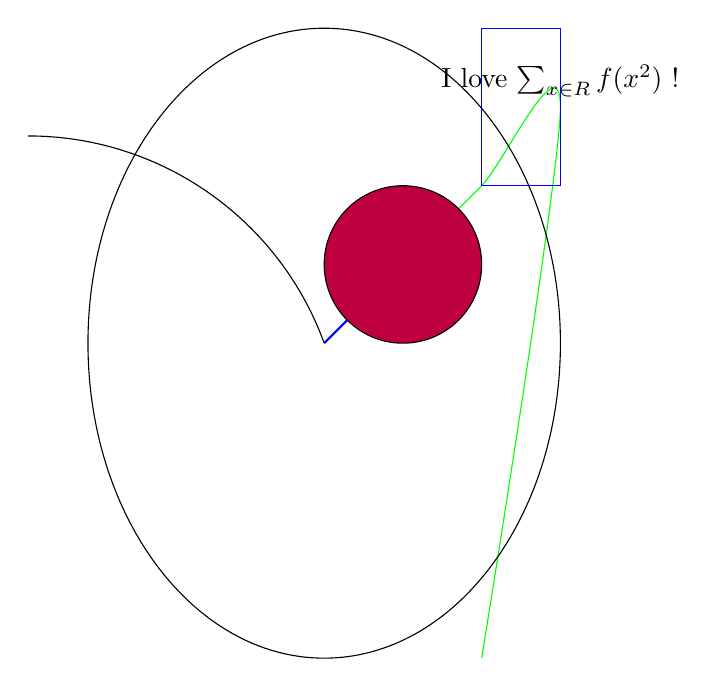
\begin{tikzpicture}[]% TikzPython id = (0) 
	\draw[thick, blue] (0, 0) .. controls (0.25, 0.25) and (0.75, 0.75)  .. (1, 1);
	\draw[green] plot[smooth ] coordinates {(1, 1) (2, 2) (3, 3) (2, -4) };
	\draw[fill = purple] (1, 1) circle (1cm);
	\node[above] at (3, 3) { I love $ \sum_{x \in \mathbb{R}} f(x^2)$ ! };
	\draw[Blue] (2, 2) rectangle (3, 4);
	\draw (0, 0) ellipse (3cm and 4cm);
	\draw (0, 0) arc (20:90:4cm);
\end{tikzpicture}
\begin{tikzpicture}[]% TikzPython id = (1) 
	\draw[Blue] plot[smooth cycle, tension = 0.5] coordinates {(2, 2) (4, 0) (1, -3) (-2, -1) (-1, 3) };
\end{tikzpicture}
